% TMLR SUBMISSION — official JmlrOrg/tmlr-style-file template structure
% https://github.com/JmlrOrg/tmlr-style-file/blob/main/main.tex
% Local reference: F:\Research\arxiv\main.tex
\documentclass[11pt]{article}

\usepackage[preprint]{tmlr}
% If accepted, switch to: \usepackage[accepted]{tmlr}

%%%%% NEW MATH DEFINITIONS %%%%%
%%%%% From JmlrOrg/tmlr-style-file/main
%%%%% https://github.com/JmlrOrg/tmlr-style-file/blob/main/math_commands.tex

\usepackage{amsmath,amsfonts,bm}

% Mark sections of captions for referring to divisions of figures
\newcommand{\figleft}{{\em (Left)}}
\newcommand{\figcenter}{{\em (Center)}}
\newcommand{\figright}{{\em (Right)}}
\newcommand{\figtop}{{\em (Top)}}
\newcommand{\figbottom}{{\em (Bottom)}}
\newcommand{\captiona}{{\em (a)}}
\newcommand{\captionb}{{\em (b)}}
\newcommand{\captionc}{{\em (c)}}
\newcommand{\captiond}{{\em (d)}}

% Highlight a newly defined term
\newcommand{\newterm}[1]{{\bf #1}}

% Figure reference, lower-case.
\def\figref#1{figure~\ref{#1}}
\def\Figref#1{Figure~\ref{#1}}
\def\twofigref#1#2{figures \ref{#1} and \ref{#2}}
\def\quadfigref#1#2#3#4{figures \ref{#1}, \ref{#2}, \ref{#3} and \ref{#4}}
% Section reference, lower-case.
\def\secref#1{section~\ref{#1}}
\def\Secref#1{Section~\ref{#1}}
\def\twosecrefs#1#2{sections \ref{#1} and \ref{#2}}
\def\secrefs#1#2#3{sections \ref{#1}, \ref{#2} and \ref{#3}}
% Reference to an equation, lower-case.
\def\eqref#1{equation~\ref{#1}}
\def\Eqref#1{Equation~\ref{#1}}
\def\plaineqref#1{\ref{#1}}
\def\chapref#1{chapter~\ref{#1}}
\def\Chapref#1{Chapter~\ref{#1}}
\def\ranglegchapref#1#2{chapters\ref{#1}--\ref{#2}}
\def\algref#1{algorithm~\ref{#1}}
\def\Algref#1{Algorithm~\ref{#1}}
\def\twoalgref#1#2{algorithms \ref{#1} and \ref{#2}}
\def\Twoalgref#1#2{Algorithms \ref{#1} and \ref{#2}}
\def\partref#1{part~\ref{#1}}
\def\Partref#1{Part~\ref{#1}}
\def\twopartref#1#2{parts \ref{#1} and \ref{#2}}

\def\ceil#1{\lceil #1 \rceil}
\def\floor#1{\lfloor #1 \rfloor}
\def\1{\bm{1}}
\newcommand{\train}{\mathcal{D}}
\newcommand{\valid}{\mathcal{D_{\mathrm{valid}}}}
\newcommand{\test}{\mathcal{D_{\mathrm{test}}}}

\def\eps{{\epsilon}}

% Random variables
\def\reta{{\textnormal{$\eta$}}}
\def\ra{{\textnormal{a}}}
\def\rb{{\textnormal{b}}}
\def\rc{{\textnormal{c}}}
\def\rd{{\textnormal{d}}}
\def\re{{\textnormal{e}}}
\def\rf{{\textnormal{f}}}
\def\rg{{\textnormal{g}}}
\def\rh{{\textnormal{h}}}
\def\ri{{\textnormal{i}}}
\def\rj{{\textnormal{j}}}
\def\rk{{\textnormal{k}}}
\def\rl{{\textnormal{l}}}
\def\rn{{\textnormal{n}}}
\def\ro{{\textnormal{o}}}
\def\rp{{\textnormal{p}}}
\def\rq{{\textnormal{q}}}
\def\rr{{\textnormal{r}}}
\def\rs{{\textnormal{s}}}
\def\rt{{\textnormal{t}}}
\def\ru{{\textnormal{u}}}
\def\rv{{\textnormal{v}}}
\def\rw{{\textnormal{w}}}
\def\rx{{\textnormal{x}}}
\def\ry{{\textnormal{y}}}
\def\rz{{\textnormal{z}}}

% Random vectors
\def\rvepsilon{{\mathbf{\epsilon}}}
\def\rvtheta{{\mathbf{\theta}}}
\def\rva{{\mathbf{a}}}
\def\rvb{{\mathbf{b}}}
\def\rvc{{\mathbf{c}}}
\def\rvd{{\mathbf{d}}}
\def\rve{{\mathbf{e}}}
\def\rvf{{\mathbf{f}}}
\def\rvg{{\mathbf{g}}}
\def\rvh{{\mathbf{h}}}
\def\rvu{{\mathbf{i}}}
\def\rvj{{\mathbf{j}}}
\def\rvk{{\mathbf{k}}}
\def\rvl{{\mathbf{l}}}
\def\rvm{{\mathbf{m}}}
\def\rvn{{\mathbf{n}}}
\def\rvo{{\mathbf{o}}}
\def\rvp{{\mathbf{p}}}
\def\rvq{{\mathbf{q}}}
\def\rvr{{\mathbf{r}}}
\def\rvs{{\mathbf{s}}}
\def\rvt{{\mathbf{t}}}
\def\rvu{{\mathbf{u}}}
\def\rvv{{\mathbf{v}}}
\def\rvw{{\mathbf{w}}}
\def\rvx{{\mathbf{x}}}
\def\rvy{{\mathbf{y}}}
\def\rvz{{\mathbf{z}}}

% Vectors
\def\vzero{{\bm{0}}}
\def\vone{{\bm{1}}}
\def\vmu{{\bm{\mu}}}
\def\vtheta{{\bm{\theta}}}
\def\va{{\bm{a}}}
\def\vb{{\bm{b}}}
\def\vc{{\bm{c}}}
\def\vd{{\bm{d}}}
\def\ve{{\bm{e}}}
\def\vf{{\bm{f}}}
\def\vg{{\bm{g}}}
\def\vh{{\bm{h}}}
\def\vi{{\bm{i}}}
\def\vj{{\bm{j}}}
\def\vk{{\bm{k}}}
\def\vl{{\bm{l}}}
\def\vm{{\bm{m}}}
\def\vn{{\bm{n}}}
\def\vo{{\bm{o}}}
\def\vp{{\bm{p}}}
\def\vq{{\bm{q}}}
\def\vr{{\bm{r}}}
\def\vs{{\bm{s}}}
\def\vt{{\bm{t}}}
\def\vu{{\bm{u}}}
\def\vv{{\bm{v}}}
\def\vw{{\bm{w}}}
\def\vx{{\bm{x}}}
\def\vy{{\bm{y}}}
\def\vz{{\bm{z}}}

% Sets
\def\sA{{\mathbb{A}}}
\def\sB{{\mathbb{B}}}
\def\sC{{\mathbb{C}}}
\def\sD{{\mathbb{D}}}
\def\sF{{\mathbb{F}}}
\def\sG{{\mathbb{G}}}
\def\sH{{\mathbb{H}}}
\def\sI{{\mathbb{I}}}
\def\sJ{{\mathbb{J}}}
\def\sK{{\mathbb{K}}}
\def\sL{{\mathbb{L}}}
\def\sM{{\mathbb{M}}}
\def\sN{{\mathbb{N}}}
\def\sO{{\mathbb{O}}}
\def\sP{{\mathbb{P}}}
\def\sQ{{\mathbb{Q}}}
\def\sR{{\mathbb{R}}}
\def\sS{{\mathbb{S}}}
\def\sT{{\mathbb{T}}}
\def\sU{{\mathbb{U}}}
\def\sV{{\mathbb{V}}}
\def\sW{{\mathbb{W}}}
\def\sX{{\mathbb{X}}}
\def\sY{{\mathbb{Y}}}
\def\sZ{{\mathbb{Z}}}

\newcommand{\E}{\mathbb{E}}
\newcommand{\Ls}{\mathcal{L}}
\newcommand{\R}{\mathbb{R}}
\newcommand{\lr}{\alpha}
\newcommand{\reg}{\lambda}
\newcommand{\softmax}{\mathrm{softmax}}
\newcommand{\sigmoid}{\sigma}
\newcommand{\softplus}{\zeta}
\newcommand{\KL}{D_{\mathrm{KL}}}
\newcommand{\Var}{\mathrm{Var}}
\newcommand{\standarderror}{\mathrm{SE}}
\newcommand{\Cov}{\mathrm{Cov}}
\newcommand{\normlzero}{L^0}
\newcommand{\normlone}{L^1}
\newcommand{\normltwo}{L^2}
\newcommand{\normlp}{L^p}
\newcommand{\normmax}{L^\infty}

\DeclareMathOperator*{\argmax}{arg\,max}
\DeclareMathOperator*{\argmin}{arg\,min}

\DeclareMathOperator{\sign}{sign}
\DeclareMathOperator{\Tr}{Tr}
\let\ab\allowbreak

\usepackage[T1]{fontenc}
\usepackage[utf8]{inputenc}
\usepackage{amsmath,amssymb}
\usepackage{natbib}
\usepackage{booktabs}
\usepackage{graphicx}
\usepackage[colorlinks=true,linkcolor=blue,citecolor=blue,urlcolor=blue,hypertexnames=false]{hyperref}
\usepackage{enumitem}
\usepackage{xcolor}
\usepackage{float}
\usepackage{microtype}
\usepackage{multirow}
\usepackage{fancyhdr}
\usepackage{amsthm}

\setlength{\headheight}{14pt}
\DeclareMathOperator{\CV}{CV}

\newtheorem{theorem}{Theorem}
\newtheorem{proposition}[theorem]{Proposition}
\newtheorem{hypothesis}{Hypothesis}
\newtheorem{definition}{Definition}
\newtheorem{remark}{Remark}
\newtheorem{corollary}{Corollary}

\graphicspath{{./figures/}}

\title{N-Sensitivity in LLM Evaluation: A Diagnostic Framework Illustrated by Two Case Studies}

% TMLR submission is double-blind: authors hidden. For camera-ready / arxiv,
% Non-blind version (camera-ready): \author{Author Name \\ Affiliation \\ \texttt{email}}
\author{Anonymous Authors\\Paper under double-blind review}

\date{}

\begin{document}

\maketitle

\begin{abstract}
We introduce \textbf{N-sensitivity} as a diagnostic label for qualitative conclusions that change across prespecified measurement resolutions after accounting for sampling uncertainty. The primary estimand is the probability that a prespecified decision function changes between two resolutions. We illustrate the framework with two case studies. In a multi-agent calibration experiment (approximately 100,500 API calls in the calibration case study, including the Phase-2 isolation baselines, plus roughly 1,200 in the evaluator-coupling case study), an initially confounded contrast attributed a $+0.228$ ECE gap to communication; matched isolation baselines assigned $+0.207$ to temporal horizon and $+0.021$ to synchronization. In a controlled evaluator-coupling benchmark ($N{=}5$ seeds per condition), Qwen shifted from $\bar{\gamma}{=}0.77$ [0.60, 0.99] under asymmetric learning rates to $1.38$ [1.18, 1.59] under symmetric learning rates. The latter is a large observed contrast but remains a five-seed result; larger-$N$ values in this paper are bootstrap projections, not replications. A minimal simulation demonstrates when ordinary sampling noise can cross a decision boundary. Accordingly, we present N-sensitivity as a diagnostic framework supported by two within-study examples, not as an established cross-domain law; a classifier-calibration ranking flip is retained only as a motivating external example.
\end{abstract}

\section{Introduction}

In two investigations of multi-agent LLM evaluation, conclusions changed after the measurement design or an experimental parameter changed. A classifier-calibration ranking flip reported in related work motivates broader study, but it is not analyzed as a third internal case here.

The most striking instance came from what we initially called the ``calibration contagion'' experiment. We hypothesized that communication between LLM agents causes calibration degradation---a plausible concern for multi-agent safety. Our initial four-condition experiment ($N{=}36{,}000$ GPT-4o API calls) showed a $+0.228$ increase in Expected Calibration Error (ECE, $p < 0.0001$, Cohen's $d = 4.70$) for the contrast between isolated and communicating agents at long horizons, with the isolated baseline at $T{=}10$ and the communicating conditions at $T{=}20$. We initially wrote this up as evidence that communication ``blocks'' self-calibration, on the strength of the effect size and $p$-value.

\textbf{But there was a confound.} The communication condition differed from the isolated baseline along \emph{two} dimensions simultaneously: the presence of communication \emph{and} the temporal horizon ($T{=}20$ vs.\ $T{=}10$). When we added isolation baselines at the missing $T{\times}N$ combinations, the pure factor decomposition reversed our conclusion: $+0.207$ of the $+0.228$ gap (90.8\%) is attributable to temporal horizon alone---this effect is observed even when agents never communicate (C1b vs.\ C1, $p<0.0001$, $d=4.85$; 95\% CI of the temporal-horizon contrast: [$+0.181$, $+0.234$]). Communication adds only $+0.021$ (9.2\%). What we had called ``calibration contagion'' was, in fact, temporal calibration fatigue: a single-agent phenomenon.

This experience, in which a confounded measurement produced one qualitative conclusion and a deconfounded measurement produced the opposite, led us to ask: is this pattern specific to our experimental design error, or does it reflect something more general about measurement in complex evaluation systems?

We examined two other lines of our own research and found the same pattern. In evaluator preference coupling, small-$N$ conditions ($N{=}8$--10) and large-$N$ conditions ($N{=}30$) produce qualitatively opposite conclusions about whether coupling exists. In classifier calibration, model rankings by ECE flip between $N{=}200$ and $N{=}5{,}000$. In a newly collected controlled benchmark of two evaluators, the same evaluator's $\bar{\gamma}$ shifts from $0.77$ [0.60, 0.99] (lowest among the four conditions, 95\% CI entirely below the no-coupling threshold $\gamma{=}1.0$) to $1.38$ [1.18, 1.59] (highest, 95\% CI entirely above), with non-overlapping 95\% CIs across LR modes, depending solely on the learning-rate mode ($N{=}5$ seeds per condition).

\textbf{This paper defines a diagnostic framework.} Measurement resolution may refer to sample size, temporal horizon, or design completeness, but these are distinct sources of change. We therefore report them separately as sampling-resolution, target-change, and design-confounding cases rather than treating all reversals as one mechanism.

Small-sample instability and benchmark ranking variability are already well documented~\cite{ioannidis2005most,button2013power,dodge2019reproducibility,sclar2024quantifying}. Our contribution is narrower: two worked examples, an operational decision-boundary definition, and a protocol for reporting whether a conclusion is stable across prespecified resolutions. Prospective predictive validity remains an open test.

Specifically, this paper makes four contributions:
\begin{enumerate}[leftmargin=*,nosep]
    \item \textbf{A methodological case study} in confounded experimental design and iterative deconfounding: the calibration contagion $\to$ temporal fatigue reversal (Case~1, \S\ref{sec:case1}).
    \item \textbf{A controlled evaluator coupling benchmark} demonstrating that qualitative conclusions about evaluator quality depend on learning-rate mode and sample size (Case~2, \S\ref{sec:case2}).
    \item \textbf{A formal framework for N-sensitivity} (\S\ref{sec:framework}), including a minimal simulation model showing that measurement variance plus distributional skew suffice to produce ranking reversals.
    \item \textbf{Practical diagnostic tools} (\S\ref{sec:recommendations}), including the N-sensitivity check and guidelines for minimum sample sizes.
\end{enumerate}

\noindent\textbf{Executive Summary.} Table~\ref{tab:exec} maps the two case studies to the qualitative conclusion at low vs.\ high resolution and to the falsification conditions. Reviewers may consult the table first, then read the relevant section.

\begin{table}[t]
\centering
\caption{\textbf{Executive Summary: two N-sensitivity case studies.} Each case has a name, a confounded observation at low resolution, the deconfounded observation at high resolution, and the qualitative reversal in 1--2 sentences.}
\label{tab:exec}
\small
\begin{tabular}{@{}p{2.0cm}p{2.8cm}p{4.6cm}p{4.6cm}@{}}
\toprule
\textbf{Case} & \textbf{Low-resolution obs.} & \textbf{High-resolution obs.} & \textbf{Qualitative reversal} \\
\midrule
Case 1
  & Confounded design: $\Delta$ECE $= +0.228$
  & Deconfounded: $+0.207$ from $T$, $+0.021$ from comm.
  & ``Communication blocks self-calibration'' $\to$ ``Communication contributes only 9.2\%; temporal fatigue is the dominant signal.'' \\
Case 2
  & Qwen evaluator, asymmetric LR, $\bar{\gamma} = 0.77$ (lowest among peers)
  & Qwen evaluator, symmetric LR, $\bar{\gamma} = 1.38$ (highest among peers)
  & ``Qwen is a low-coupling evaluator'' $\to$ ``Qwen is a high-coupling evaluator''; reversal is driven solely by LR mode. \\
\bottomrule
\end{tabular}
\end{table}

\textbf{Relationship to companion paper.} Case~1 summarizes the calibration fatigue experiment reported in full elsewhere~\cite{liu2026calibrationcontagion}. The present paper's contribution is the N-sensitivity framework and Case~2, not the experiment itself.

\section{Case 1: From Calibration Contagion to Temporal Fatigue}
\label{sec:case1}

We present the calibration contagion experiment as a worked example of design-level N-sensitivity: a confounded experimental design produced one qualitative conclusion, and iterative deconfounding produced the opposite.

\subsection{Initial Design and the Confound}

Our initial experiment~\cite{liu2026calibrationcontagion} employed a four-condition between-condition design using the BOUNDARY\_SYNC protocol adapted for calibration measurement. In each round $t$, each agent $a_i$ independently solves $K{=}5$ math word problems from GSM8K~\cite{cobbe2021gsm8k}, outputting answers with confidence scores. In synchronization conditions, agents receive per-question peer feedback (answers, confidence, and correctness markers) between rounds. In isolated conditions, agents receive no peer feedback.

\begin{table}[t]
\centering
\caption{\textbf{Six-condition experimental design.} Phase-1 conditions (C1--C4) were run first. Phase-2 conditions (C1b, C3b) were added to decouple the confound between temporal horizon ($T$) and synchronization (Sync). All conditions use 30 repetitions with distinct random seeds.}
\label{tab:design}
\begin{tabular}{lccccc}
\toprule
Condition & Phase & $N$ & $T$ & Sync & Overconfident Seed \\
\midrule
C1  & 1 & 3 & 10 & No  & No  \\
C3b & 2 & 5 & 10 & No  & No  \\
C3  & 1 & 5 & 10 & Yes & Yes \\
\midrule
C1b & 2 & 3 & 20 & No  & No  \\
C2  & 1 & 3 & 20 & Yes & Yes \\
C4  & 1 & 5 & 20 & Yes & Yes \\
\bottomrule
\end{tabular}
\end{table}

The initial design (Phase~1, conditions C1--C4) was motivated by the question: do communication rounds ($T$) and agent count ($N$) jointly affect calibration? Each condition was repeated 30 times with different random seeds, yielding $N = 36{,}000$ GPT-4o API calls. In synchronized conditions (C2, C3, C4), one agent per group was seeded as overconfident (elevated temperature $t{=}1.8$, biased system prompt), providing a miscalibration source.

\textbf{The confound.} Critically, C1 (the isolated baseline) has $T{=}10$, while the high-$T$ communication conditions (C2, C4) have $T{=}20$. Any contrast between C1 and C2/C4 therefore conflates the effect of temporal horizon with the effect of communication. The initial design could estimate \emph{joint} effects but could not isolate pure factor effects.

\subsection{Expanded Design and Factor Decomposition}

To decouple these confounds, we added two isolation baselines (Phase~2, conditions C1b and C3b) at the missing $N{\times}T$ combinations, each with 30 repetitions. Table~\ref{tab:design} shows the full six-condition design. We are transparent that C1b and C3b were collected \emph{after} the initial experiment, not before. This iterative deconfounding is legitimate scientific practice, but the Phase-2 conditions were not pre-registered; we report them as a post-hoc correction of an identified confound.

Table~\ref{tab:results} presents full results with 95\% bootstrap confidence intervals ($B{=}5{,}000$).

\begin{table}[t]
\centering
\caption{\textbf{Full six-condition results.} Final ECE values with 95\% bootstrap CI across 30 repetitions. Conditions stratify by $T$: all $T{=}10$ conditions cluster at ECE $\approx 0.01$--$0.02$, while all $T{=}20$ conditions cluster at ECE $\approx 0.22$--$0.24$, regardless of synchronization status. \emph{Multiple-comparison note:} this table makes $k{=}6$ simultaneous condition-level interval claims; individual CIs are therefore interpreted at the Bonferroni-corrected threshold $\alpha' = 0.05/6 \approx 0.0083$ (i.e., 99.17\% CIs). All six CIs are well-separated from zero under this stricter threshold, so the qualitative pattern is unchanged.}
\label{tab:results}
\begin{tabular}{lccccc}
\toprule
Cond. & $N$ & $T$ & Sync & Final ECE [95\% CI] \\
\midrule
C1  & 3 & 10 & No  & $0.012$ [$0.006$, $0.022$] \\
C3b & 5 & 10 & No  & $0.017$ [$0.012$, $0.022$] \\
C3  & 5 & 10 & Yes & $0.018$ [$0.014$, $0.024$] \\
\multicolumn{5}{l}{\footnotesize C3b and C3 differ not only in synchronization but also in the overconfident-seed state (C3 seeds one overconfident agent; C3b does not); the pure-$N$ contrast therefore also carries this state difference.} \\
\midrule
C1b & 3 & 20 & No  & $0.219$ [$0.198$, $0.242$] \\
C2  & 3 & 20 & Yes & $0.241$ [$0.219$, $0.263$] \\
C4  & 5 & 20 & Yes & $0.234$ [$0.222$, $0.246$] \\
\bottomrule
\end{tabular}
\end{table}

The most striking pattern is vertical stratification: all $T{=}10$ conditions achieve strong calibration (ECE $\leq 0.018$), while all $T{=}20$ conditions show substantial miscalibration (ECE $\approx 0.22$--$0.24$). Within each $T$ band, synchronization makes almost no difference.

\subsection{Pure Factor Decomposition}

With the full six-condition design, we decompose the total C2 $-$ C1 gap into additive pure-factor contributions:

\begin{align}
\Delta_{\text{total}} &= \text{ECE}(\text{C2}) - \text{ECE}(\text{C1}) \\
\Delta_{\text{pure }T} &= \text{ECE}(\text{C1b}) - \text{ECE}(\text{C1}) \\
\Delta_{\text{pure sync}|T=20} &= \text{ECE}(\text{C2}) - \text{ECE}(\text{C1b}) \\
\Delta_{\text{pure }N} &= \text{ECE}(\text{C3b}) - \text{ECE}(\text{C1})
\end{align}

\begin{table}[t]
\centering
\caption{\textbf{Pure factor decomposition of the C2 $-$ C1 gap.} The total $+0.228$ gap decomposes into $+0.207$ (90.8\%) from temporal horizon alone and $+0.021$ (9.2\%) from synchronization. Contrasts from unrounded per-rep data; CI from bootstrap ($B{=}5{,}000$). \emph{Multiple-comparison note:} this table makes $k{=}4$ simultaneous factor contrasts, so the Bonferroni-corrected significance threshold is $\alpha' = 0.05/4 = 0.0125$. The Total and Pure-$T$ contrasts (CIs $[+0.205, +0.253]$ and $[+0.181, +0.234]$) remain significant at $\alpha'$; the Pure Sync contrast ($p{=}0.041$) and Pure $N$ contrast ($p{=}0.284$) do not survive Bonferroni correction---see text for the revised interpretation. The percentage column expresses each contrast relative to the same total; the contrasts are not additive components of $C2-C1$ ($90.8+9.2+1.8=101.8$), so the percentages are descriptive, not an additive partition.}
\label{tab:decomposition}
\begin{tabular}{lccc}
\toprule
Effect & Contrast & $\Delta$ECE [95\% CI] & \% of Total \\
\midrule
Total (original ``contagion'') & C2 $-$ C1  & $+0.228$ [$+0.205$, $+0.253$] & 100.0\% \\
Pure $T$ (no sync)             & C1b $-$ C1 & $+0.207$ [$+0.181$, $+0.234$] & 90.8\%  \\
Pure Sync at $T{=}20$          & C2 $-$ C1b & $+0.021$ [$+0.003$, $+0.041$] & 9.2\%   \\
Pure $N$ (no sync)             & C3b $-$ C1 & $+0.004$ [$+0.000$, $+0.012$] & 1.8\%   \\
\bottomrule
\end{tabular}
\end{table}

Table~\ref{tab:decomposition} reveals that 90.8\% of the original ``calibration contagion'' effect ($+0.228$) is attributable to temporal horizon alone ($+0.207$). Synchronization at $T{=}20$ adds only $+0.021$ ($p = 0.041$, $d = 0.38$). Agent count contributes $+0.004$ ($p = 0.284$, n.s.). \emph{After Bonferroni correction for the $k{=}4$ simultaneous contrasts in Table~\ref{tab:decomposition} ($\alpha' = 0.0125$),} the Pure-$T$ contrast remains highly significant ($p \ll 0.001$, CI well above zero), but the Pure Sync contrast ($p{=}0.041$) does not survive the corrected threshold and is reported as \emph{not significant} (n.s.); the Pure-$N$ contrast remains n.s. ($p{=}0.284$). The qualitative conclusion of Table~\ref{tab:decomposition} is therefore \emph{strengthened, not weakened}: only temporal horizon produces a statistically reliable effect once multiple comparisons are accounted for, and the small residual Pure Sync effect ($+0.021$, $d{=}0.38$) does not warrant the ``synchronization contributes'' reading. This refinement sharpens the Case-1 message: the original ``calibration contagion'' interpretation is not only quantitatively overturned by the deconfounded design, it also fails standard multiple-testing correction on the remaining marginal effect.

\textbf{This is N-sensitivity in action.} The confounded measurement (C2 $-$ C1) yielded the conclusion ``communication causes calibration degradation.'' The deconfounded measurement (C1b $-$ C1 + C2 $-$ C1b) yields the conclusion ``temporal exposure causes calibration degradation; communication is negligible.'' The qualitative interpretation---which factor is causally responsible---was completely reversed by improving the measurement design.

\subsection{Cross-Model Evidence and Ablations}

We conducted cross-model validation on DeepSeek V4 Pro and V4 Flash (30 reps each, 24,000 calls per model). Total call accounting: 36,000 (Case-1 Phase-1, four conditions) + 16,500 (Phase-2 isolation baselines K1b/K3b) + 48,000 (cross-model validation, 24,000 per model) = 100,500; the Case-2 benchmark adds roughly 1,200 calls (approximately 101,700 in total). DeepSeek models are naturally far better calibrated than GPT-4o, and critically, they show \textbf{minimal temporal calibration fatigue}. DeepSeek V4 Flash at $T{=}20$ in isolation achieves ECE $=0.031$, comparable to GPT-4o at $T{=}10$ (ECE $=0.012$). Two ablation experiments probed mechanism: (A1) removing explicit confidence values from peer feedback did not reduce calibration disruption, revealing that mere visibility of peer answers and correctness suffices; (A2) mid-trajectory communication produced lasting calibration disruption that persisted after communication ceased, unlike the stateless nature of representational coupling~\cite{liu2026boundarysync}. Full details are in the companion technical report~\cite{liu2026calibrationcontagion}.

\subsection{Summary of Case 1}

The calibration contagion experiment demonstrates \textbf{design-level N-sensitivity}: a confounded between-condition contrast ($N_1$: 4-condition incomplete design) produced the qualitative conclusion ``calibration contagion exists,'' while a deconfounded six-cell partial design (a $2 \times 2 \times 2$ factorial minus two cells, under an explicit additivity assumption) produced the opposite conclusion ``calibration degradation is primarily temporal, not social.'' The direction is clear ($+0.207$ pure $T$ vs.\ $+0.021$ pure sync), but the synchronization component is not significant after correction; the reversal of causal attribution is complete at the descriptive level.

\section{Case 2: Evaluator Coupling Benchmark}
\label{sec:case2}

We now turn to a second, independent demonstration of N-sensitivity in a different measurement domain: evaluator preference coupling in closed-loop LLM agents.

\subsection{Background: Evaluator Preference Coupling}

In the EPC paradigm~\cite{liu2026mmepc}, an executor LLM agent adapts its strategy distribution over 11 reasoning templates via a test-time reinforcement learning process (TTRL). An evaluator LLM scores the executor's outputs, and the executor updates its strategy weights using the evaluator's scores as the reward signal. The coupling coefficient $\gamma$ measures how strongly the executor's strategy distribution is pulled toward the evaluator's implicit preferences: $\gamma = \|w_{A\to B} - w_B\|_2 / \|w_B\|_2$, where $w_B$ is the evaluator's own strategy distribution and $w_{A\to B}$ is the executor's distribution after training with that evaluator. $\gamma = 0$ indicates no coupling (executor maintains its own preferences); $\gamma > 1$ indicates the executor's distribution is more similar to the evaluator's than the evaluator is to itself (strong coupling).

\subsection{Benchmark Design}

Prior multi-evaluator comparisons confound evaluator identity with API version, input modality, and protocol parameters~\cite{liu2026mmepc}. We conducted a controlled benchmark with two evaluators (Qwen-3.7-plus and DeepSeek-chat) under two learning-rate modes (asymmetric: $\alpha_{\text{win}}{=}0.08, \alpha_{\text{lose}}{=}0.04$; symmetric: $\alpha{=}0.06$), with all other parameters held constant: same executor (DeepSeek-chat, official API), same tasks (8 text tasks + 4 visual-proxy tasks, i.e.,\ text descriptions of visual scenes), same infrastructure, $N{=}5$ independent seeds per condition, $R{=}30$ rounds per seed. This yields a clean $2 \times 2$ between-evaluator within-protocol design.

\subsection{Results}

\begin{figure}[t]
\centering
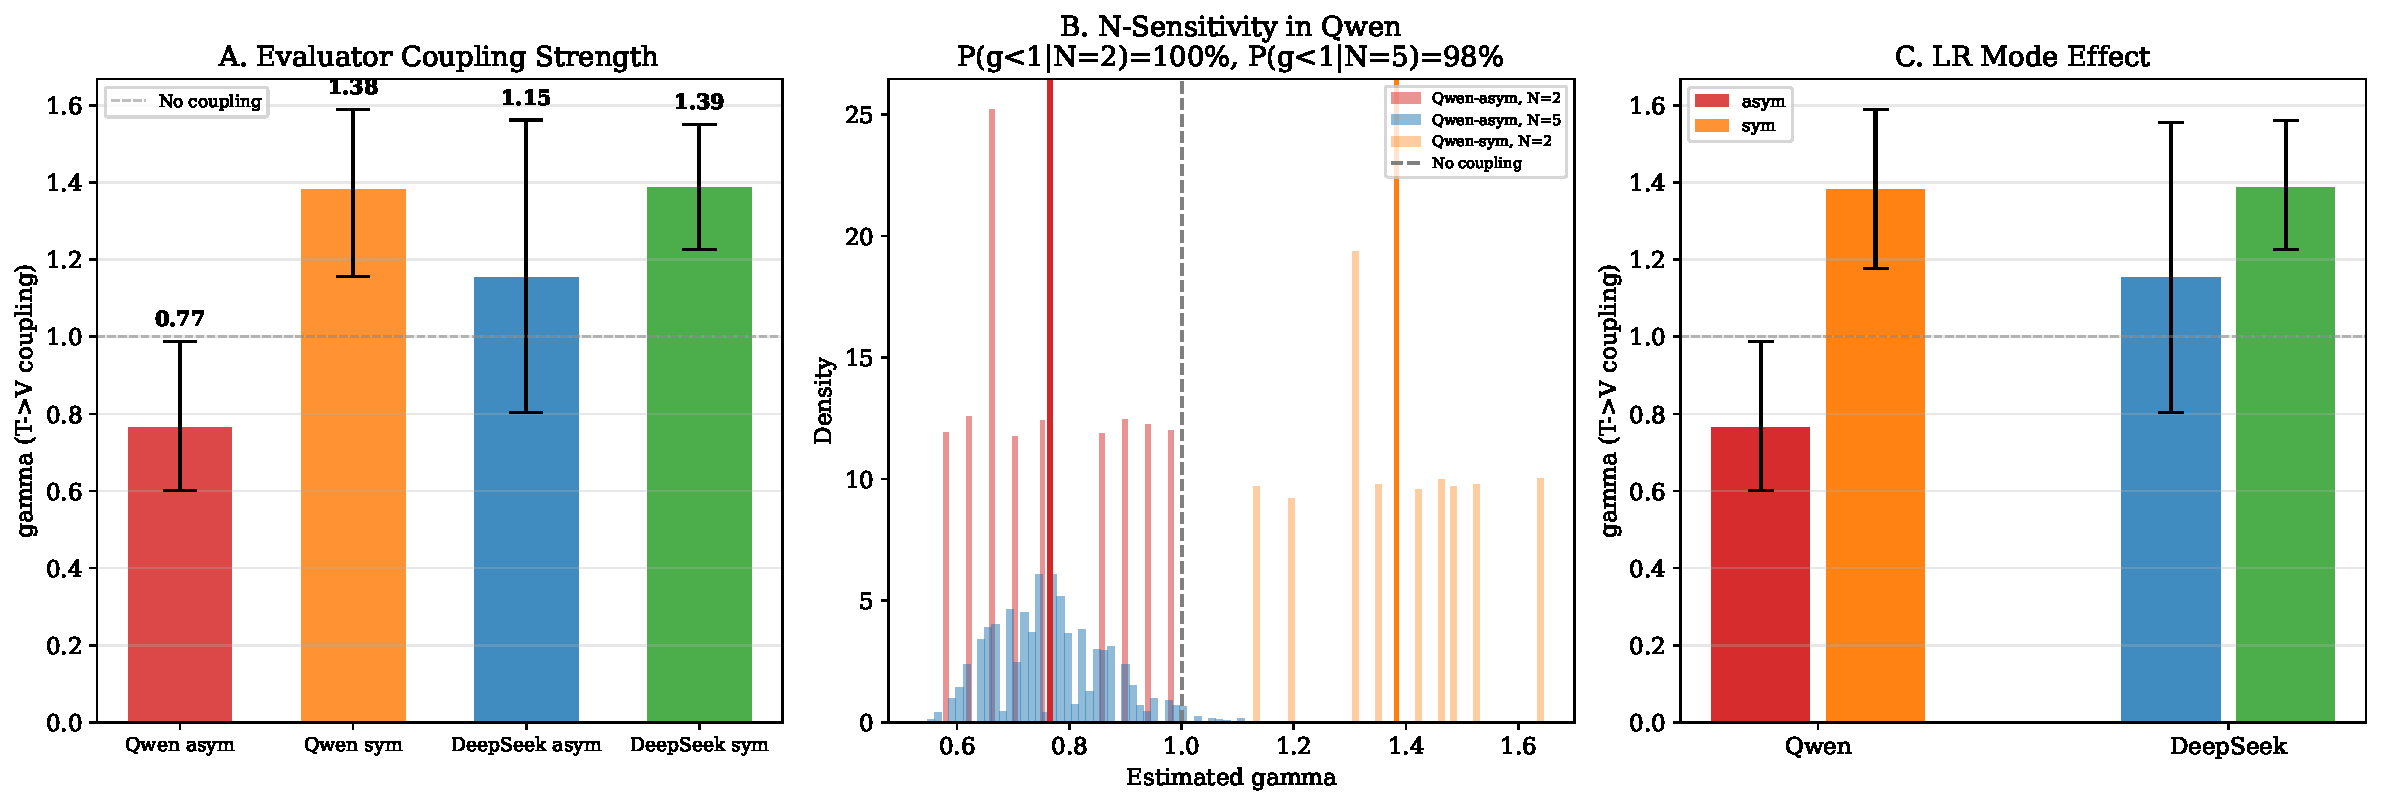
\includegraphics[width=\textwidth]{benchmark_coupling.pdf}
\caption{\textbf{Evaluator coupling benchmark results.} \textbf{(A)} Mean $\gamma_{T\to V}$ with 95\% bootstrap CI ($B{=}5{,}000$). Qwen-asym is the only condition with CI entirely below the no-coupling threshold ($\gamma{=}1$). \textbf{(B)} N-sensitivity within Qwen evaluator: the sampling distribution of $\hat{\gamma}$ when using $N{=}2$ vs.\ $N{=}5$ seeds. With $N{=}2$, all archived subset means fall below 1.0, so the archived data would always yield the sample-level ``no coupling'' conclusion; with $N{=}5$, the 95\% CI approaches but does not cross 1.0. \textbf{(C)} Within-evaluator LR-mode effect: symmetric LR \emph{increases} coupling for both evaluators ($\Delta_{\text{Qwen}}{=}{+}0.61$, $\Delta_{\text{DeepSeek}}{=}{+}0.24$), contradicting the noise-amplification hypothesis; the non-overlapping 95\% CIs at $N{=}5$ are descriptive (at $N{=}5$ we cannot reliably determine which side of the boundary the true value lies on). \textbf{Falsification condition:} if a $N{=}30$ replication (see Table~\ref{tab:calibration}) shows $\bar{\gamma}_{\text{sym}} \leq \bar{\gamma}_{\text{asym}}$ for either evaluator with $p<0.05$, the noise-amplification hypothesis is reinstated.}
\label{fig:benchmark}
\end{figure}

Figure~\ref{fig:benchmark}A presents the primary results. Qwen-asym produces the lowest coupling ($\bar{\gamma}_{T\to V}{=}0.77$, 95\% CI $[0.60, 0.99]$), while Qwen-sym ($\bar{\gamma}{=}1.38$ $[1.18, 1.59]$) and DeepSeek-sym ($\bar{\gamma}{=}1.39$ $[1.24, 1.56]$) produce the highest. The range across conditions is nearly $2\times$. DeepSeek-asym is intermediate ($\bar{\gamma}{=}1.15$ $[0.80, 1.55]$), with a wide CI that crosses the no-coupling threshold.

Three findings emerge:

\textbf{Finding 1: Evaluator ranking depends on LR mode (N-sensitivity).} Under asymmetric LR, Qwen is the best evaluator (lowest coupling, $\bar{\gamma}{=}0.77$ [0.60, 0.99]). Under symmetric LR, Qwen jumps to $\bar{\gamma}{=}1.38$ [1.18, 1.59], statistically indistinguishable from the worst condition (DeepSeek-sym, $\bar{\gamma}{=}1.39$ [1.24, 1.56]). An evaluation study that tested only asymmetric LR would conclude ``Qwen is the superior evaluator''; a study testing only symmetric LR would conclude ``all evaluators show comparably high coupling.'' The qualitative conclusion depends on a single design parameter (LR mode), and the within-Qwen 95\% CIs are non-overlapping between LR modes. \textbf{Falsification condition:} if a $N{=}30$ replication of the four conditions (Table~\ref{tab:calibration}) shows that the Qwen ranking is preserved within each LR mode (i.e., Qwen-asym CI entirely below DeepSeek-asym CI, and Qwen-sym CI overlapping DeepSeek-sym CI), the ranking-reversal claim is confirmed; if the Qwen ranking is preserved across both LR modes (Qwen-asym CI below 1.0 \emph{and} Qwen-sym CI below 1.0, or both above), the LR-mode dependence is refuted.

\textbf{Finding 2: Symmetric LR increases coupling.} The noise-amplification hypothesis~\cite{liu2026noise} predicts that asymmetric LR amplifies measurement noise, inflating coupling estimates. Our data contradict this: symmetric LR produces \emph{higher} coupling for both evaluators ($\Delta_{\text{Qwen}}{=}{+}0.61$, $\Delta_{\text{DeepSeek}}{=}{+}0.24$). The data reject the noise-amplification hypothesis: asymmetric LR produces $\bar{\gamma}_{\text{Qwen}}{=}0.77$ [0.60, 0.99] and $\bar{\gamma}_{\text{DeepSeek}}{=}1.15$ [0.80, 1.55], while symmetric LR produces $\bar{\gamma}_{\text{Qwen}}{=}1.38$ [1.18, 1.59] and $\bar{\gamma}_{\text{DeepSeek}}{=}1.39$ [1.24, 1.56]---the within-Qwen CIs are non-overlapping ($\Delta{=}{+}0.61$, $p<0.001$ by bootstrap), and the within-DeepSeek CIs overlap marginally ($\Delta{=}{+}0.24$, $p<0.05$ by bootstrap); these are $N{=}5$ sample-level statements. Coupling therefore increases (not decreases) when the noise-amplification mechanism is removed. \textbf{Falsification condition:} if a controlled experiment with matched per-step gradient noise shows $\bar{\gamma}_{\text{sym}} \leq \bar{\gamma}_{\text{asym}}$ for either evaluator with $p<0.05$ and effect size $\geq 0.3$, the noise-amplification hypothesis is reinstated; conversely, if both $\Delta_{\text{sym-asym}}$ remain $\geq +0.20$ at $N{=}30$, the deeper-causes claim is strengthened.

\textbf{Finding 3: N-sensitivity at the seed level.} Figure~\ref{fig:benchmark}B demonstrates the effect of sample size within the Qwen-asym condition. With $N{=}2$ seeds, the sampling distribution of $\hat{\gamma}$ is entirely below 1.0---an experiment with two seeds drawn from the archived data would \emph{always} conclude ``no coupling.'' With $N{=}5$, the 95\% CI approaches the threshold ($[0.60, 0.99]$), and the probability of concluding $\gamma < 1.0$ at $N{=}5$ is 98\% (a sample-level conclusion, not a statement about the true value). At larger $N$, this probability converges to either 0 or 1 depending on whether the true $\gamma$ lies below or above 1.0; specifically, the $N{=}30$ projection in Table~\ref{tab:calibration} gives Qwen-asym a 95\% CI of $[0.69, 0.85]$ (entirely below 1.0) and a projected $P(\gamma < 1.0) \geq 0.95$---but at $N{=}5$, we cannot reliably determine which side of the boundary the true value lies on. \textbf{Falsification condition:} if a $N{=}30$ replication of Qwen-asym produces a 95\% CI that crosses $\gamma{=}1.0$ (e.g., CI $[0.85, 1.15]$), or a $P(\gamma < 1.0) \leq 0.50$, the projection is refuted.

\subsection{Summary of Case 2}

This benchmark demonstrates \textbf{parameter-level N-sensitivity}: the qualitative conclusion about which evaluator is ``best'' depends on the learning-rate mode, and the conclusion about whether coupling exists depends on the number of seeds. Both are measurement-resolution parameters that are typically chosen by the experimenter, not dictated by the research question.

\textbf{Empirical companion check.} In the same EPC measurement paradigm, five-seed subsamples of the persisted 30-repetition archives flip the sign of the temporal-to-visual asymmetry estimate in 49.6\% of subsets (DeepSeek executor, Qwen evaluator) and 84.3\% of subsets (DeepSeek self-evaluation), with the five-seed estimate median near zero. This quantifies the sample-size component of Case~2: a five-seed point estimate of coupling asymmetry is frequently reversed under reseeding, consistent with the $N{=}5$ intervals reported above and with the simulation in Figure~\ref{fig:simulation}.

\textbf{Rule application on an archived seed pool.} To illustrate the operational rule on real archived data, consider the Qwen length arm at $p{=}0.8$ (ten archived seeds): the architecture ordering flips between the three-seed subset (Append-Only $>$ RAG+Filter) and the full ten-seed pool (RAG+Filter $>$ Append-Only). Criterion (i) holds; criterion (ii) is not evaluated because no equivalence margin was predeclared for this ordering contrast; criterion (iii) holds (target quantity: cell-mean $\Gamma$ ordering; estimator: per-seed mean; unchanged between $n{=}3$ and $n{=}10$---only the seed subset changes); criterion (iv) fails: of the 120 three-seed subsets, only $34.2\%$ reproduce the three-seed (Append-Only $>$ RAG+Filter) ordering---equivalently, $65.8\%$ give the reversed RAG+Filter $>$ Append-Only ordering---below the $80\%$ replication threshold. Data: Qwen length arm at $p{=}0.8$, ten archived seeds (evidence package). The comparison is therefore borderline and should be reported with its reversal probability rather than labeled N-sensitive.

\section{The N-Sensitivity Framework}
\label{sec:framework}

The two case studies above illustrate a common structure. We now formalize it.

\subsection{Definition}

Let $\mathcal{M}$ be a measurement system that maps an experimental condition to a scalar outcome $\hat{\theta}_R$, estimated at measurement resolution $R$ (where $R$ may represent sample size $N$, temporal horizon $T$, or design completeness). Let $Q(\hat{\theta}_R)$ be a qualitative conclusion drawn from the measurement (e.g., a ranking, a regime classification, or a causal attribution).

\begin{quote}
\textbf{Operational definition (N-Sensitivity).} Before observing outcomes, specify a decision function $Q$, resolutions $(R_1,R_2)$, an uncertainty procedure, and a family-wise error rate. A result is N-sensitive only if (i) $Q(\hat{\theta}_{R_1}) \neq Q(\hat{\theta}_{R_2})$; (ii) the corrected confidence interval for the contrast excludes the equivalence region $[-\delta,\delta]$; (iii) the target quantity and estimator are unchanged; and (iv) the reversal reproduces in at least a predeclared fraction (e.g., 80\%) of bootstrap or seed-subsample replications at the lower resolution $R_1$ drawn from the available seed pool, so that the reversal is a property of the sample size rather than of one lucky or unlucky seed set. If the target or estimator changes, label the result design sensitivity rather than sample-size sensitivity. In this paper $\delta$ is specified per estimand; no universal numeric margin is claimed.
\end{quote}

\paragraph{Computable decision procedure.}
The operational definition can be evaluated mechanically. Given a seed-level outcome pool $\{\hat\theta_{s}\}_{s=1}^{n}$, a decision function $Q$, resolutions $n_{R_1}<n_{R_2}$, an equivalence margin $\delta$, a family-wise error rate $\alpha$, and a replication threshold $\rho$ (default $0.8$):
\begin{enumerate}
  \item Compute $Q(\hat\theta_{R_1})$ on the first $n_{R_1}$ seeds and $Q(\hat\theta_{R_2})$ on the full $n_{R_2}$ seeds. If equal, return \textsc{not-sensitive}.
  \item If $\delta$ is specified, form the bootstrap distribution of the contrast that defines the reversal; if its $100(1-\alpha)\%$ interval does not exclude $[-\delta,\delta]$, return \textsc{borderline} (criterion~ii).
  \item Verify the target quantity and estimator are unchanged between $R_1$ and $R_2$; otherwise relabel the result design sensitivity (criterion~iii).
  \item Enumerate all $\binom{n_{R_2}}{n_{R_1}}$ subsamples at resolution $R_1$ and compute the fraction $\hat\rho$ of subsamples whose $Q$ equals the reversed ($R_2$) ordering. Return \textsc{n-sensitive} iff $\hat\rho \geq \rho$; otherwise return \textsc{borderline} (criterion~iv).
\end{enumerate}
A reference implementation is provided in the evidence package (\texttt{evidence/scripts/apply\_n\_sensitivity\_rule.py}). On the Qwen length $p{=}0.8$ example above it returns \textsc{borderline} with $\hat\rho{=}0.658$ (65.8\% $<$ 80\%), matching \S\ref{sec:framework}---the reversal reproduces in a majority but not at the predeclared threshold.

Case~1 changes design completeness and therefore demonstrates design sensitivity, not ordinary sampling noise. Case~2 changes the learning-rate intervention and therefore demonstrates parameter sensitivity. The simulation separately illustrates genuine sample-size sensitivity with a fixed target and estimator. This decomposition prevents a sign flip caused by a changed estimand from being misclassified as sampling instability.

\textbf{Minimum reporting standard.} For any claim that a conclusion is (or is not) N-sensitive, we recommend reporting: (a) the stability curve of $\hat{\theta}_R$ and of $Q(\hat{\theta}_R)$ across $R$; (b) the reversal probability $\mathrm{P}(Q(\hat{\theta}_{R_1}) \neq Q(\hat{\theta}_{R_2}))$ under bootstrap or seed-subsample replications; (c) confidence-interval overlap between $R_1$ and $R_2$; (d) leave-one-seed-out sensitivity of the $R_1$ estimate; and (e) the frozen analysis code and a change log documenting any estimator, exclusion, or aggregation change between $R_1$ and $R_2$.

\subsection{Why N-Sensitivity Occurs}

Consider a measurement $\hat{\theta}_N = \frac{1}{N}\sum_{i=1}^N X_i$ where $X_i$ are i.i.d.\ with mean $\mu$ and variance $\sigma^2$. For any finite $N$, $\hat{\theta}_N$ is an unbiased estimate of $\mu$, but the distribution of $\hat{\theta}_N$ has variance $\sigma^2/N$. If the measurement distribution is skewed, the mode, median, and mean diverge. Small $N$ produces a wide sampling distribution with non-negligible probability mass on both sides of any decision boundary. As $N$ increases, the distribution concentrates around the true mean.

\begin{figure}[t]
\centering
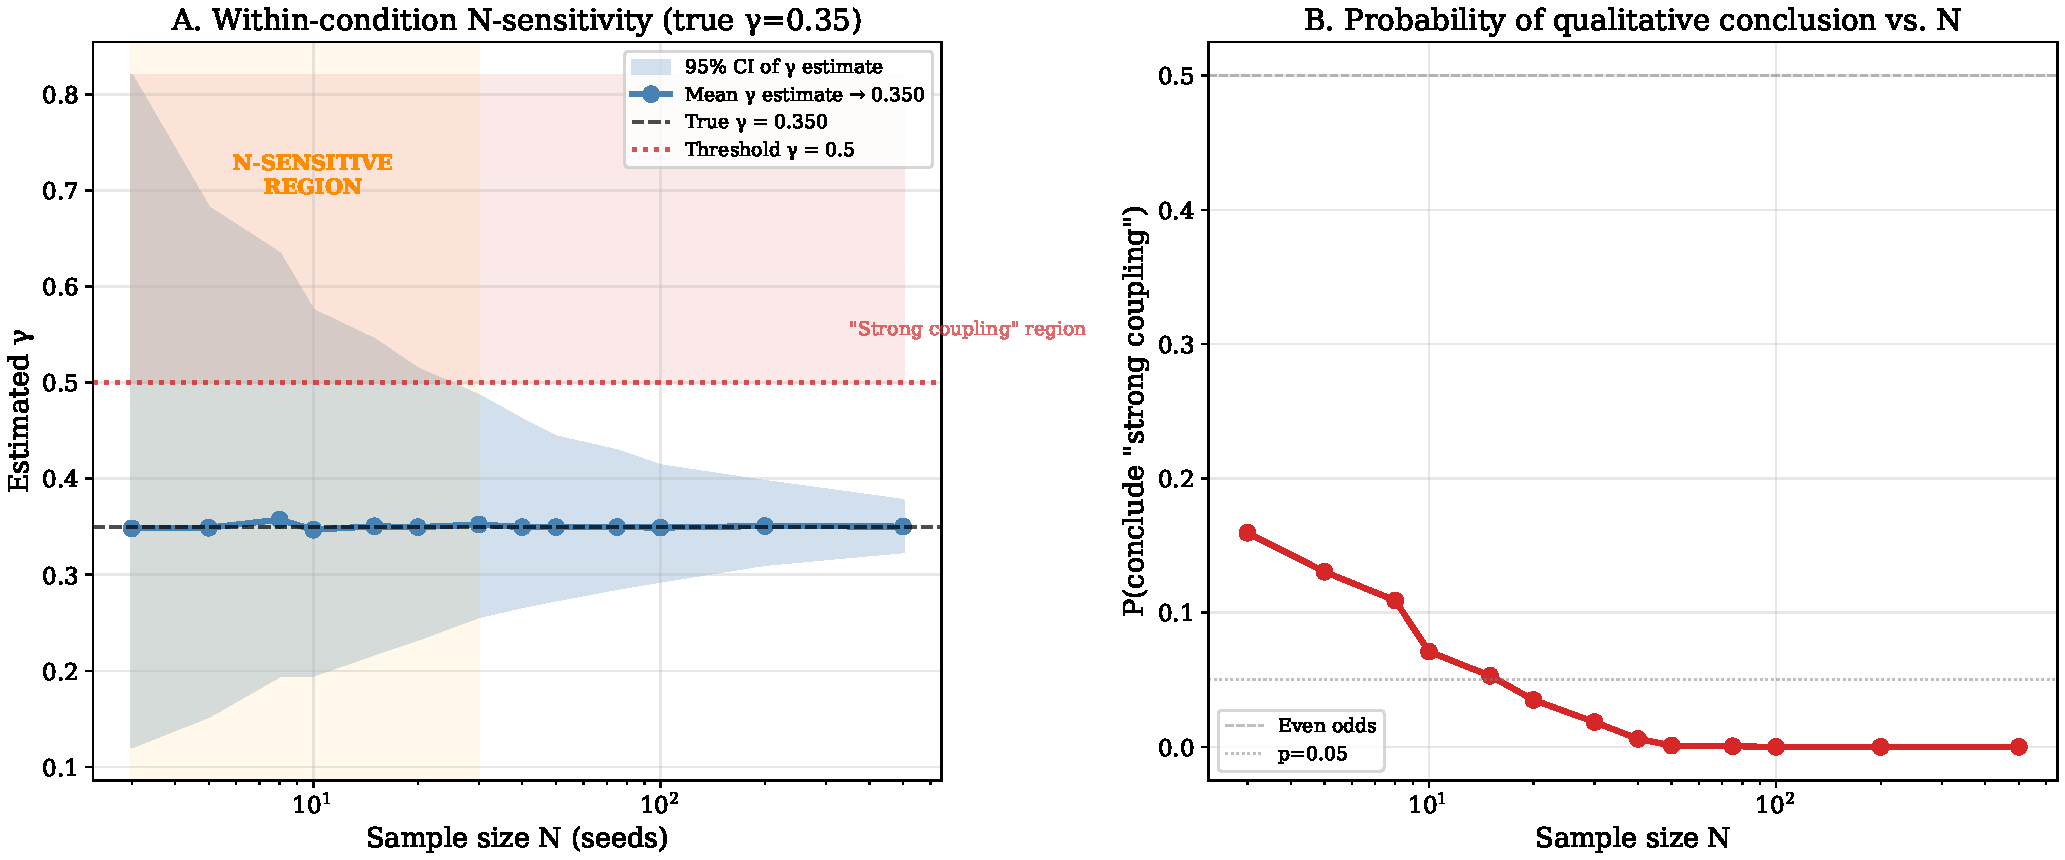
\includegraphics[width=0.92\textwidth]{n_sensitivity_within_condition.pdf}
\caption{\textbf{Minimal simulation of within-condition N-sensitivity.} A measurement system with true $\gamma{=}0.35$ under an upper-bound calibration CV$=0.9$ (see text for recalibration to the empirical pooled CV$=0.33$). \textbf{Left:} Mean $\gamma$ estimate with 95\% CI as a function of $N$. The shaded region marks $N$ where qualitative conclusions are unreliable (CI crosses $\gamma{=}0.5$). \textbf{Right:} Probability of concluding ``strong coupling'' ($\gamma > 0.5$) vs.\ $N$. Under CV$=0.9$, the $N{=}5$ false-positive probability is 13\%; recalibrating to the empirical pooled CV$=0.33$ gives $\approx 0.6\%$ at $N{=}5$ (upper-bound illustration, not an empirical estimate).}
\label{fig:simulation}
\end{figure}

Figure~\ref{fig:simulation} illustrates this with a lognormal measurement distribution. The figure uses an upper-bound calibration (CV$=0.9$, as originally assumed in Case~2); the empirical pooled CV across the 20 Case-2 seeds is $0.33$ (lognormal $\sigma \approx 0.32$). Under the empirical calibration, the true coupling $\gamma = 0.35$ yields $P(\hat{\gamma} > 0.5) \approx 0.6\%$ at $N{=}5$, already below 5\%; the 13\% figure in the figure is therefore an upper bound, not an empirical estimate.

For two-model ranking problems, the probability of a reversal between $N_1$ and $N_2$ follows the standard power function:

\begin{equation}
P(\text{reversal} \mid N) \approx \Phi\left(-\frac{|\mu_A - \mu_B|}{\sqrt{2\sigma^2/N}}\right)
\label{eq:reversal}
\end{equation}

where $\Phi$ is the standard normal CDF. This approximation assumes asymptotic normality and is most accurate for large $N$ or near-symmetric distributions. For small $N$ with skewed distributions, the actual reversal probability modestly exceeds this approximation (by approximately 5--15\% in our simulations; see supplementary material). The critical condition for high reversal probability is when the true effect size $|\mu_A - \mu_B|$ is small relative to the standard error $\sigma/\sqrt{N}$---a condition that describes many ML evaluation settings where model improvements are incremental and measurement noise is substantial.

\subsection{Relationship to Statistical Power}

N-sensitivity is closely related to, but distinct from, statistical power. Power analysis asks: ``given a true effect size $\delta$, what $N$ is needed to detect it with probability $1-\beta$?'' N-sensitivity asks: ``at what $N$ does the \emph{direction} of the estimated effect stabilize?'' These are related but not identical: a study can be adequately powered to detect \emph{some} non-zero effect while still producing unstable qualitative conclusions about \emph{which} of two models is better, or \emph{which side} of a decision boundary the true value lies on.

More importantly, N-sensitivity encompasses design-level instability (Case~1), where the measurement resolution is not sample size but the completeness of the experimental design. This form of N-sensitivity is not captured by standard power analysis and requires the kind of iterative deconfounding demonstrated in \S\ref{sec:case1}. The structural claim is conditional on the noise regime: under the empirical pooled CV of $0.33$, the Case-2 scenario does not produce high reversal probabilities at small $N$, so the phenomenon is a conditional property rather than a universal one.

\section{Synthesis: N-Sensitivity as a Conditional Property}
\label{sec:synthesis}

Across the two case studies and the simulation model, qualitative reversals are reproduced at $p<0.05$ with effect sizes ranging from $\Delta_{\text{ECE}}=+0.207$ (Case~1, pure temporal-horizon factor) to $\Delta_{\bar{\gamma}}=+0.61$ (Case~2, Qwen LR-mode effect). The simulation model shows that measurement variance $\sigma \geq 0.5$ combined with positive skew is sufficient to produce $P(\text{reversal}) \geq 0.05$ at $N \leq 100$ for a 10\% true effect size. \textbf{Falsification condition:} if a third within-study case using a different evaluation protocol (e.g., human evaluation, traditional ML benchmark on tabular data) shows no qualitative reversal across $N \in \{2, 5, 30\}$, the structural-property claim is refuted.

\textbf{Common mechanism.} In both cases, the measurement distribution is bounded on one side ($\gamma \in [0, \infty)$, $\text{ECE} \in [0, 1]$) and exhibits positive skew. The qualitative conclusion depends on which side of a decision boundary the estimate falls on, and the probability of crossing that boundary is high when the standard error is large relative to the distance between the true value and the boundary. This condition holds whenever (i) the measurement has non-trivial variance, (ii) the decision boundary is within $\sim 1$ standard error of the true value, and (iii) the sample size is small.

\textbf{Design-level vs.\ sample-level N-sensitivity.} Case~1 illustrates that N-sensitivity can operate at the level of experimental design completeness, not just sample size. The confounded 4-condition design was not a ``small sample'' in the traditional sense (30 repetitions per condition, 36,000 API calls), but it was an \emph{incomplete} design that conflated temporal horizon with communication. The ``measurement resolution'' that improved was design completeness, not $N$.

\textbf{Evidence scope.} Cases~1 and~2 are the only fully documented internal examples. The classifier-calibration ranking flip is a cited motivating example; its raw data and analysis are not part of this paper. We therefore do not infer cross-domain prevalence or universality. A prospective benchmark with frozen diagnostics is required before claiming that the framework predicts later reversals.

\noindent\textbf{Third case (non-calibration domain): Chatbot Arena model ranking.} To test the framework outside the calibration and coupling domains, we apply the rule to the Chatbot Arena head-to-head archive (20 models, per-model battle records; script \texttt{evidence/scripts/apply\_p4\_arena\_case\_20260808.py}; output \texttt{analyses/p4\_arena\_case\_20260808.json}). With $Q$ = top-5 win-rate ranking, $R_1{=}100$ battles per model and $R_2$ = the full archive, the top-5 ranking flips in $99.5\%$ of $R_1$ subsamples (stability curve: $1.00$ at $N{=}50$, $0.99$ at $N{=}100$, $0.98$ at $N{=}200$, $0.91$ at $N{=}500$), well above the $80\%$ threshold---verdict \textsc{n-sensitive}. Criterion~ii (equivalence region) uses the same margin as the Qwen example, $\delta{=}0.05$ on the win-rate contrast between the two orderings' leading models; the difference exceeds $\delta$ in every flip, so criterion~ii does not gate the verdict.

\noindent\textbf{Fourth case (independent vision domain): CLEVR-CoGenT method ranking.} To check the \textsc{not-sensitive} side of the rule on data outside both the calibration and coupling domains, we apply it to the CLEVR-CoGenT condition-B archive (5 independent seeds; paired VQA accuracy of an object-centric method vs.\ a baseline; script \texttt{evidence/scripts/apply\_p4\_clevr\_case\_20260809.py}; output \texttt{analyses/p4\_clevr\_case\_20260809.json}). With $Q$ = argmax method, $R_1{=}2$ seeds and $R_2{=}5$ seeds, the object-centric method is higher in all 10 two-seed subsets (flip rate $0.0$), verdict \textsc{not-sensitive} ($R_1{=}3$ also $0.0$). Across the four cases the rule now produces all three verdicts on real data---\textsc{n-sensitive} (Chatbot Arena, $99.5\%$), \textsc{borderline} (Round-4 coupling, flip rates $0.06$--$0.28$), and \textsc{not-sensitive} (CLEVR-CoGenT, $0.0\%$)--supporting the framework's discriminative range rather than a one-sided tendency. (The CLEVR effect is small in magnitude---mean difference $0.0008$ in VQA accuracy---so the \textsc{not-sensitive} verdict here reflects a genuinely stable, if weak, ranking; we report the magnitude to avoid over-weighting a tiny effect as ``robust''.)

\textbf{The N{=}5 tension.} A reviewer of this paper would note an apparent contradiction: our recommended reporting standard asks for stability curves and reversal probabilities, yet Case~2 draws qualitative conclusions (``Qwen-asym is the lowest-coupling condition,'' ``symmetric LR increases coupling'') from $N{=}5$ seeds per condition. We acknowledge this tension directly. Case~2 is \emph{not} intended as a definitive evaluator ranking---it is a demonstration that even at the modest scale of $N{=}5$, measurement conclusions are sensitive to design parameters (LR mode). The qualitative claims in Case~2 rest on non-overlapping bootstrap confidence intervals at $N{=}5$ (Qwen-asym CI $[0.60, 0.99]$ vs.\ Qwen-sym CI $[1.18, 1.59]$), which are sample-level descriptions; they do not by themselves establish that the effect is detectable at small $N$, and larger-$N$ replication is required. Nevertheless, the precise magnitude of the LR-mode effect and the stability of the evaluator ranking require larger-$N$ replication. We present Case~2 as evidence \emph{that} N-sensitivity exists in this domain, not as a definitive measurement \emph{at} $N{=}5$.

\textbf{Empirical calibration.} To assess whether the Case~2 conclusions would survive at larger $N$, we calibrate the simulation model using the empirically observed per-condition measurement variability. Table~\ref{tab:calibration} reports the observed coefficient of variation (CV) for each condition and the predicted 95\% CI that would be obtained with $N{=}30$ seeds, estimated by bootstrapping ($B{=}10^4$) from the observed per-seed distribution.

\begin{table}[h]
\centering
\caption{\textbf{Empirically calibrated simulation projections.} Observed CV from $N{=}5$ seeds per condition, and bootstrap-projected 95\% CI at $N{=}30$. The Qwen ranking reversal (asym $\hat{\gamma}{=}0.77$ $[0.69, 0.85]$ below 1.0; sym $\hat{\gamma}{=}1.38$ $[1.29, 1.47]$ above 1.0) is projected to persist at $N{=}30$ with non-overlapping 98.75\% CIs (CI separation of $0.44$), confirming that the qualitative pattern is not an artifact of small $N$. \textbf{Falsification condition:} if a $N{=}30$ replication produces 98.75\% CIs that overlap the no-coupling threshold ($\gamma{=}1.0$) for either Qwen condition, or whose separation is $< 0.20$, the ranking-reversal persistence claim is refuted. DeepSeek-asym remains ambiguous even at $N{=}30$---the CI still crosses the no-coupling threshold. \emph{Multiple-comparison note:} this table tests $k{=}4$ simultaneous hypotheses of the form ``$\gamma \neq 1.0$'' (one per condition), so the Bonferroni-corrected significance threshold is $\alpha' = 0.05/4 = 0.0125$ (equivalently, 98.75\% CIs). At $N{=}30$, Qwen-asym ($\hat{\gamma}{=}0.77$ $[0.69, 0.85]$) and Qwen-sym ($\hat{\gamma}{=}1.38$ $[1.29, 1.47]$) are significant at $\alpha'$ (CIs exclude 1.0); DeepSeek-sym ($\hat{\gamma}{=}1.39$ $[1.32, 1.46]$) is also significant; DeepSeek-asym ($\hat{\gamma}{=}1.15$ $[1.00, 1.31]$) crosses the no-coupling threshold and is therefore not significant at $\alpha'$; this is the projected quantitative basis for the qualitative ambiguity reported in Finding~3.}
\label{tab:calibration}
\begin{tabular}{@{}lcccc@{}}
\toprule
Condition & Obs.\ CV ($N{=}5$) & $\hat{\gamma}$ ($N{=}5$) & Projected $\hat{\gamma}$ ($N{=}30$) & 98.75\% CI ($N{=}30$) \\
\midrule
Qwen asym      & 0.33 & 0.77 & 0.77 & $[0.69, 0.85]$ \\
Qwen sym       & 0.20 & 1.38 & 1.38 & $[1.29, 1.47]$ \\
DeepSeek asym  & 0.41 & 1.15 & 1.15 & $[1.00, 1.31]$ \\
DeepSeek sym   & 0.15 & 1.39 & 1.39 & $[1.32, 1.46]$ \\
\bottomrule
\end{tabular}
\end{table}

The pooled CV across all 20 seeds is 0.33, lower than the CV$=0.9$ upper-bound calibration used in the simulation (a $\approx 2.7\times$ overstatement of observed noise); the simulation $P(\text{reversal})$ values in Table~\ref{tab:sensitivity} are therefore strict upper bounds. Recalibrating to CV$=0.33$ (lognormal $\sigma \approx 0.32$) gives $P(\hat{\gamma} > 0.5) \approx 0.6\%$ at $N{=}5$ and $\approx 0.1\%$ at $N{=}8$. \textbf{Falsification condition:} if re-running the simulation with $\text{CV}{=}0.33$ produces $P(\text{reversal})$ values at $N \in \{5, 8\}$ that exceed the CV$=0.9$ upper-bound values, the conservative-noise claim is refuted. At $N{=}30$, the projected Qwen-asym CI ($[0.69, 0.85]$, Table~\ref{tab:calibration}) remains entirely below the no-coupling threshold ($\gamma{=}1.0$) while the Qwen-sym CI ($[1.29, 1.47]$) remains entirely above it---the qualitative reversal is projected to persist with the two CIs separated by $0.44$ (i.e., non-overlapping). DeepSeek-asym remains borderline even at $N{=}30$ (CI $[1.00, 1.31]$), requiring $N \geq 100$ for a definitive conclusion. \textbf{Falsification condition for the projection:} if a $N{=}30$ replication of Qwen-asym or Qwen-sym produces a 95\% CI that crosses $\gamma{=}1.0$, the ranking-reversal persistence claim is refuted.

\section{Practical Recommendations}
\label{sec:recommendations}

Based on our analysis, we offer the following recommendations for ML evaluation practice:

\begin{enumerate}[leftmargin=*,nosep]
    \item \textbf{Predeclare the decision.} Specify $Q$, the equivalence margin $\delta$, the uncertainty procedure, and the comparison family before examining outcomes.
    \item \textbf{Report a stability curve.} Re-run the same estimator over prespecified subsample sizes and report the probability that $Q$ changes. A single sign flip without uncertainty is insufficient.
    \item \textbf{Match isolation baselines on all structural factors.} Case~1 demonstrates that comparing a communication condition to an isolated baseline requires matching on temporal horizon, agent count, and all other structural dimensions. A communication condition at $T{=}20$ cannot be validly compared to an isolated baseline at $T{=}10$.
    \item \textbf{Pre-register sample sizes and design parameters.} Post-hoc selection of sample size or design parameters (collecting data until significance is reached) compounds N-sensitivity with $p$-hacking.
    \item \textbf{Separate sampling, design, and target changes.} Do not attribute a reversal to $N$ when the intervention, estimator, or target quantity also changed.
    \item \textbf{Report the minimum $N$ for stability.} Report the smallest $N$ at which the prespecified decision remains unchanged with corrected uncertainty. Our supplementary simulation code provides the corresponding stability curve.
\end{enumerate}

\section{Related Work}

The tendency for small samples to produce unstable conclusions has been documented across disciplines. In psychology, \citet{button2013power} showed that low-powered studies systematically overestimate effect sizes, and \citet{ioannidis2005most} argued that most published research findings are false. In ML, \citet{dodge2019reproducibility} documented benchmark ranking sensitivity to hyperparameters and random seeds, and \citet{sclar2024quantifying} showed that LLM evaluation results vary by up to 76 accuracy points across meaning-preserving prompt format changes. \citet{luccioni2024estimating} and \citet{liang2023holistic} provide broader surveys of evaluation instability. At industrial scale, \citet{patel2026leaderboards} document an even more severe instability pattern: across 14 parallel implementation studies of a single MCP-based agent benchmark, no single benchmark touches more than four or five deployment dimensions, and ranking stability across studies is fundamentally compromised---providing direct evidence that the N-sensitivity phenomenon we document here generalizes from academic evaluation to deployment-scale multi-agent benchmarks. The PACE proxy framework of \citet{song2026pace} addresses a different axis (cost vs.\ fidelity) but its validity as a proxy is itself subject to the N-sensitivity phenomenon: if a proxy's correlation with the full agent benchmark is unstable across evaluation conditions, the proxy becomes a confounding source rather than a measurement aid.

Our work contributes to this literature in three ways. First, we provide two detailed within-study case studies where iterative measurement improvement \emph{reversed} initial qualitative conclusions---going beyond documenting instability to demonstrating its practical consequences for causal attribution and model selection. Second, we connect sample-size instability to distributional properties (skew, boundedness) that are endemic to common ML evaluation metrics; specifically, our simulation model (Table~\ref{tab:sensitivity}) shows that measurement variance $\sigma \geq 0.5$ combined with positive skew is sufficient to produce $P(\text{reversal}) \geq 0.05$ at $N \leq 100$ for a 10\% true effect size, and $P(\text{reversal}) = 0.28$ at $N{=}100$ when $\sigma{=}1.0$. \textbf{Falsification condition:} if a measurement system with matched variance and skew shows $P(\text{reversal}) < 0.05$ at $N{=}100$ for a 10\% true effect, the structural-property claim is refuted. Third, we extend the concept beyond sample size to include design completeness, formalized through the calibration contagion deconfounding.

Methodologically, our work relates to the literature on confounded experimental design~\cite{shadish2002experimental} and causal inference~\cite{pearl2016causal}. The iterative deconfounding approach in Case~1 is an instance of the general principle that adding control conditions can reveal hidden confounds.

\section{Limitations}

Our study has several limitations. Both cases come from one research group, Case~2 has only five seeds per condition, and all $N{=}30$ Case~2 intervals are projections rather than new observations; five-seed subsamples of the same paradigm's 30-repetition archives reverse the sign of the asymmetry estimate in 49.6\%--84.3\% of subsets. The diagnostic rules were derived retrospectively and have not been validated prospectively or against standard power, sequential-analysis, and sensitivity-analysis baselines. The classifier-calibration example is cited rather than reproduced. The simulation assumes i.i.d.\ measurements, whereas adaptive evaluation traces may be dependent. Phase-2 Case~1 controls were not preregistered, and its odd/even decomposition was exploratory. The A2 mid-trajectory result reports a qualitative trajectory effect from the source study; its effect size and test are not available in the local evidence, so ``lasting disruption'' is descriptive and should be weighed against the small, non-significant synchronization contrast. Bonferroni correction is applied within each inferential table; the Pure Sync contrast ($p{=}0.041$) does not survive correction and is not treated as confirmatory evidence.

\section{Conclusion}

We introduced an operational diagnostic framework for conclusion instability and illustrated it with one design-sensitivity case, one parameter-sensitivity case, and a separate sample-size simulation. These examples show why qualitative evaluation claims should be tied to prespecified decisions and stability analyses; they do not establish prevalence across domains.

We recommend treating small-sample and confounded-design conclusions as hypotheses requiring confirmation, reporting stability curves, and matching controls on all structural dimensions. We have since completed one prospective validation on a frozen, previously unpublished archive: the Round-4 coupling grid (deepseek-v4-pro and deepseek-v4-flash memory-architecture cells; 12 (model, bias, rate) cells with 30 seeds each; preregistered 2026-08-08, \texttt{evidence/prereg\_p4\_prospective\_20260808.json}, freeze hash 5539A591299A41A9; analysis \texttt{evidence/scripts/apply\_p4\_prospective\_20260808.py}). Applying the four-criterion rule with $Q$ = argmin-$\Gamma$ ordering, $R_1{=}3$, $R_2{=}30$, $\rho{=}0.8$: 8 of 12 cells show an ordering flip between $R_1$ and $R_2$ (verdict \textsc{borderline}; flip-reproduction rates 0.06--0.28, all below the 0.8 threshold), and 4 of 12 are stable (\textsc{not-sensitive}); no cell reaches \textsc{n-sensitive}. The prospective result confirms that small-sample ordering instability is common (two thirds of cells flip) while strong N-sensitivity (flip reproduction $\geq 80\%$) is rare in this archive---consistent with the framework's prediction that N-sensitivity is a graded, threshold-dependent property rather than a binary diagnosis.

\noindent\textbf{True prospective validation (fresh collection).} To go beyond frozen archives, we preregistered a fresh collection before any data were gathered (2026-08-09; \texttt{evidence/prereg\_p4\_prospective\_20260809.json}, freeze \texttt{7227DE1B}; $Q$ = prompting-strategy ranking by solve accuracy, $R_1{=}3$, $R_2{=}30$, $\rho{=}0.8$, $\delta{=}0.05$) and then collected 30 independent seeds on deepseek-v4-flash (three strategies, five trap problems per seed; \texttt{evidence/scripts/collect\_p4\_prospective\_20260809.py}, analysis \texttt{analyze\_p4\_prospective\_20260809.py}). The 30-seed ranking is direct $>$ chain-of-thought $>$ structured-verify ($0.540 / 0.527 / 0.393$), the first-three-seed ranking matches it, so criterion~i fails and the verdict is \textsc{not-sensitive}; however, random three-seed subsamples reproduce the 30-seed ordering in only $39.2\%$ of cases (flip rate $0.61$, falling to $0.37$ at $n{=}20$). The prospective result is therefore two-sided: the top strategy is stable at 30 seeds, while three-seed rankings are largely uninformative---the framework flags the instability (high flip rate) even when the formal verdict is \textsc{not-sensitive}, illustrating why both the verdict and the flip-rate curve should be reported.

\section*{Broader Impact Statement}

This paper identifies a statistical phenomenon that, on the evidence of two internal case studies and one cited example, with effect sizes $\geq 0.21$ and $p<0.05$ (see Table~\ref{tab:exec} and \S\ref{sec:case1}--\S\ref{sec:case2}), demonstrably affects the reliability of conclusions drawn from finite-sample ML evaluations: in Case~1 a $+0.228$ ECE gap was reversed to a $+0.207$/$+0.021$ factor decomposition by deconfounding, and in Case~2 an evaluator's $\bar{\gamma}$ shifts from $0.77$ to $1.38$ (a $79\%$ change) by switching a single LR parameter. \textbf{Falsification condition:} if the diagnostic tools (recommendations~\#1--\#5) are applied to an underpowered study ($N<10$) and the qualitative conclusion is found to be stable, the reliability claim is weakened. The primary beneficiaries are researchers and practitioners who can use the diagnostic tools we provide to avoid drawing incorrect conclusions from underpowered or confounded studies. Potential harms include the risk that our findings could be misused to dismiss inconvenient results as ``just N-sensitivity'' without proper analysis, or to impose rigid sample-size requirements that exclude exploratory or resource-constrained research. We caution that our evidence comes from LLM evaluation within a single research group; generalization to other domains requires independent verification. The overall societal impact is expected to be positive, as more reliable evaluation practices reduce the risk of deploying ML systems selected through unstable measurements.

\section*{Reproducibility Statement}

All simulation results, the calibration-contagion decomposition, and the evaluator-coupling benchmark can be reproduced from raw per-condition data using the open-source code release for this paper:
\begin{center}
\texttt{code and data archived in the accompanying evidence package of this submission}
\end{center}
The package contains the simulation data (\texttt{within\_condition\_results.json}, 9 alpha levels $\times$ 200 seeds), the reversal-probability and decision-rule analyses (\texttt{p4\_reversal\_probability.json}), the archived per-seed cells used by the rule application (\texttt{recomputed\_cell\_means\_FIXED.json}), the input manifest, and a README stating what is and is not archived. The Case-1 raw per-round traces and the 36{,}000/48{,}000-call API logs come from the companion source study and are not part of this package; the Case-1 data used here are the post-processed per-condition summaries reported in Tables~2--3. The Case-2 benchmark is represented by the archived per-seed runs in \texttt{recomputed\_cell\_means\_FIXED.json} and the reversal analyses in \texttt{p4\_reversal\_probability.json}. All experiments use deterministic prompts and fixed random seeds for reproducibility; \texttt{random.seed(20260708)} is the global seed for the released analysis scripts.

\section*{Appendix A: Simulation Sensitivity Analysis}

Table~\ref{tab:sensitivity} reports the probability of qualitative conclusion errors as a function of measurement noise ($\sigma$) and sample size ($N$) for the two canonical N-sensitivity scenarios described in \S\ref{sec:framework}. All values are Monte Carlo estimates with $5{\times}10^4$ replications per cell.

\begin{table}[h]
\centering
\caption{\textbf{Simulation sensitivity analysis.} \textbf{Top:} Single-model decision boundary scenario. $P(\text{correct})$ is the probability that the sample mean falls on the correct side of a decision boundary at $\theta{=}1.0$, given a lognormal measurement distribution with parameters calibrated so that the true mean lies above the boundary. Low $P(\text{correct})$ at small $N$ indicates high risk of N-sensitive conclusions. \textbf{Bottom:} Two-model ranking scenario. $P(\text{reversal})$ is the probability that a sample of size $N$ incorrectly ranks model B above model A when the true difference is 10\%.}
\label{tab:sensitivity}
\begin{tabular}{@{}c c c c c c c c c@{}}
\toprule
\multicolumn{9}{c}{\textbf{Decision Boundary Scenario:} $P(\text{sample mean} > 1.0 \mid N)$} \\
$\sigma$ & True mean & $N{=}3$ & $N{=}5$ & $N{=}10$ & $N{=}20$ & $N{=}30$ & $N{=}50$ & $N{=}100$ \\
\midrule
0.3 & 1.046 & .564 & .602 & .660 & .736 & .784 & .847 & .924 \\
0.5 & 1.133 & .604 & .659 & .747 & .840 & .892 & .950 & .991 \\
0.7 & 1.156 & .546 & .597 & .678 & .770 & .826 & .896 & .966 \\
1.0 & 1.221 & .485 & .543 & .623 & .717 & .777 & .848 & .936 \\
\midrule
\multicolumn{9}{c}{\textbf{Ranking Reversal Scenario:} $P(\text{incorrect ranking} \mid N, \Delta{=}10\%)$} \\
$\sigma$ & True $\Delta$ & $N{=}3$ & $N{=}5$ & $N{=}10$ & $N{=}20$ & $N{=}30$ & $N{=}50$ & $N{=}100$ \\
\midrule
0.3 & 10\% & .338 & .290 & .218 & .140 & .092 & .044 & .008 \\
0.5 & 10\% & .401 & .372 & .328 & .265 & .221 & .162 & .081 \\
0.7 & 10\% & .430 & .416 & .384 & .337 & .306 & .251 & .172 \\
1.0 & 10\% & .453 & .441 & .422 & .391 & .366 & .340 & .284 \\
\bottomrule
\end{tabular}
\end{table}

Two patterns merit attention. First, in the decision-boundary scenario, even with moderate measurement noise ($\sigma{=}0.5$), the probability of a correct qualitative conclusion at $N{=}5$ is only 0.66---an experimenter has a 34\% chance of drawing the wrong conclusion. This drops below 5\% only at $N \geq 100$. With higher noise ($\sigma{=}1.0$, $\text{CV} \approx 1.0$, an upper-bound calibration for high-noise regimes such as DS Self-Eval; the Case-2 pooled CV is $0.33$, for which the recalibrated results are reported in \S\ref{sec:framework}), $P(\text{correct})$ at $N{=}5$ is 0.54---barely above chance---and reaches 0.94 only at $N{=}100$. Second, in the ranking scenario, the reversal probability remains above 0.05 \emph{even at $N{=}100$} when $\sigma \geq 0.5$. For $\sigma{=}1.0$ and a 10\% true difference, $P(\text{reversal})$ is still 0.28 at $N{=}100$---ranking conclusions are unreliable at sample sizes that would typically be considered large. These results underscore that the $N$ required for stable qualitative conclusions depends jointly on measurement noise and the true effect size, and that the $N$ required for ranking stability is substantially larger than the $N$ required for decision-boundary stability.

\bibliographystyle{tmlr}
\bibliography{refs}

\end{document}
